\documentclass[a4paper, twoside]{report}

%% Language and font encodings
\usepackage[english]{babel}
\usepackage[utf8x]{inputenc}
\usepackage[T1]{fontenc}

%% Sets page size and margins
\usepackage[a4paper,top=3cm,bottom=2cm,left=3cm,right=3cm,marginparwidth=1.75cm]{geometry}

%% Useful packages
\usepackage{amsmath}
\usepackage{graphicx}
\usepackage[colorinlistoftodos]{todonotes}
%\usepackage[colorlinks=true, allcolors=blue]{hyperref}
\usepackage{url}
\usepackage{tcolorbox}
\usepackage{float}
\usepackage{setspace}

\title{Adaptive Compression for Graph Processing}
\author{Rob Moore}
% Update supervisor and other title stuff in title/title.tex

\begin{document}
\begin{titlepage}

\newcommand{\HRule}{\rule{\linewidth}{0.5mm}} % Defines a new command for the horizontal lines, change thickness here

%----------------------------------------------------------------------------------------
%	LOGO SECTION
%----------------------------------------------------------------------------------------


\includegraphics[width=8cm]{title/logo.png}\\[1cm] % Include a department/university logo - this will require the graphicx package
 
%----------------------------------------------------------------------------------------

\center % Center everything on the page

%----------------------------------------------------------------------------------------
%	HEADING SECTIONS
%----------------------------------------------------------------------------------------

\textsc{\LARGE BEng Individual Project}\\[1.5cm] % Name of your university/college
\textsc{\Large Imperial College London}\\[0.5cm] % Major heading such as course name
\textsc{\large Department of Computing}\\[0.5cm] % Minor heading such as course title

%----------------------------------------------------------------------------------------
%	TITLE SECTION
%----------------------------------------------------------------------------------------
\makeatletter
\HRule \\[0.4cm]
{ \huge \bfseries \@title}\\[0.4cm] % Title of your document
\HRule \\[1.5cm]
 
%----------------------------------------------------------------------------------------
%	AUTHOR SECTION
%----------------------------------------------------------------------------------------

\begin{minipage}{0.4\textwidth}
\begin{flushleft} \large
\emph{Author:}\\
\@author % Your name
\end{flushleft}
\end{minipage}
~
\begin{minipage}{0.4\textwidth}
\begin{flushright} \large
\emph{Supervisor:} \\
Dr. Holger Pirk \\[1.2em] % Supervisor's Name
\emph{Second Marker:} \\
Prof. Peter Pietzuch % second marker's name
\end{flushright}
\end{minipage}\\[2cm]
\makeatother

% If you don't want a supervisor, uncomment the two lines below and remove the section above
%\Large \emph{Author:}\\
%John \textsc{Smith}\\[3cm] % Your name

%----------------------------------------------------------------------------------------
%	DATE SECTION
%----------------------------------------------------------------------------------------

{\large \today}\\[2cm] % Date, change the \today to a set date if you want to be precise

\vfill % Fill the rest of the page with whitespace

\end{titlepage}

\onehalfspacing
%\doublespacing
\linespread{1.15}

\begin{abstract}
Many graph-modeled data sources are subject to fast-changing, unpredictable workloads, such as a news story being searched for as it happens, or a trending post or person on social media causing an influx of related, similar queries. Most processing frameworks for graph data sources contain preprocessing steps to speed up the overall analysis, which prohibits them from responding to queries until that step is done. In this report we explore potential solutions to this problem by building novel variations of database cracking, an algorithm designed for auto-tuning relational databases, and showing how the cracking algorithm can be changed to improve performance for graph data processing.
\end{abstract}

\renewcommand{\abstractname}{Acknowledgements}
\begin{abstract}
I would like to thank my supervisor Holger Pirk for his knowledge and direction during the project. I am also grateful to my personal tutor, Paul Kelly, for his advice about projects in general and about optimization and graph algorithms, as well as all of the interesting discussions we've had while I've been at Imperial. Finally I'd like to thank my dad who scanned the boundary pieces of this report and gave me some advice on how to improve it.
\end{abstract}

\tableofcontents
\listoffigures
\listoftables

\chapter{Introduction}

\section{Motivation and Objectives}

\section{Contributions}

\chapter{Related Work}

\label{ch:relatedwork}

\section{Workload-Aware Frameworks}

\subsection{Database Cracking}

From Idreos et al, Cracking is a relational database auto-tuning technique which performs online restructuring of a relational table into disjoint pieces, storing information about each piece within a separate data-structure called the cracker index.

When a column is queried, it is copied into a version of the column called the cracker column. The cracker column is then scanned, restructuring it in-place to position the retrieved elements in contiguous memory. The indices of the bounds of the newly formed contiguous region are stored within the cracker index to optimise future queries by reducing the amount of the column needing to be scanned.

Figure \ref{fig:cracking_img} shows two queries being run against a column within a system employing database cracking. We can see that Q1 copies the original column into a cracker column, which is then partitioned into pieces from the scan, of which information is known about the contents. Q2 further breaks up the column into pieces, and again the information about the newly formed partitions is stored in the cracker index.

\begin{figure}[h]
  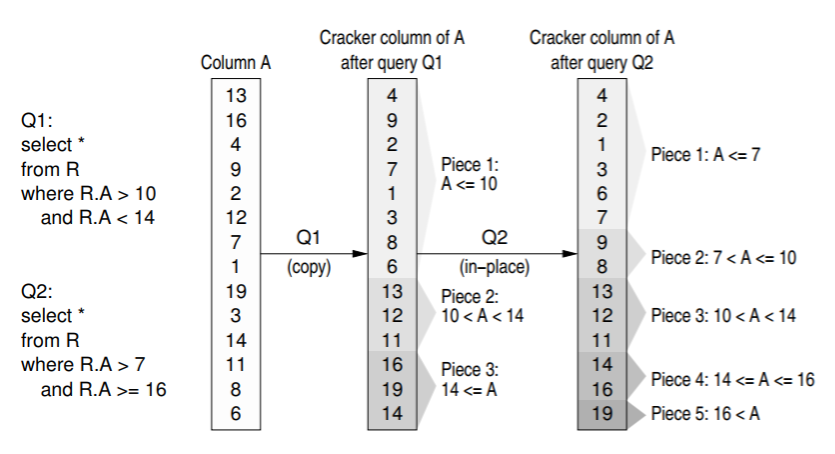
\includegraphics[width=\textwidth]{cracking_img}
  \caption{Example of a column being cracked}
  \label{fig:cracking_img}
\end{figure}

Database cracking is discussed in much more detail in Chapter \ref{ch:background}.

\subsection{Group-by-Query}

In-part inspired by cracking was the thesis work of Aluç, who proposed a group-by-query (G-by-Q) representation for RDF data, for which the structure of individual database records, as well as the way records are serialized on the storage system are dynamically determined based on the workload. 

Using G-by-Q, the way database records are serialised and their contents are determined dynamically by the workload. The format of database records is determined by the queries on the database. The diagram below shows an example of the storage for a database which has had two types of queries applied to it. $P_{1}$ to $P_{3}$ are the results of a linear query, whereas $P_{4}$ and $P_{5}$ are both the results of star-shaped queries.

\begin{figure}[h]
  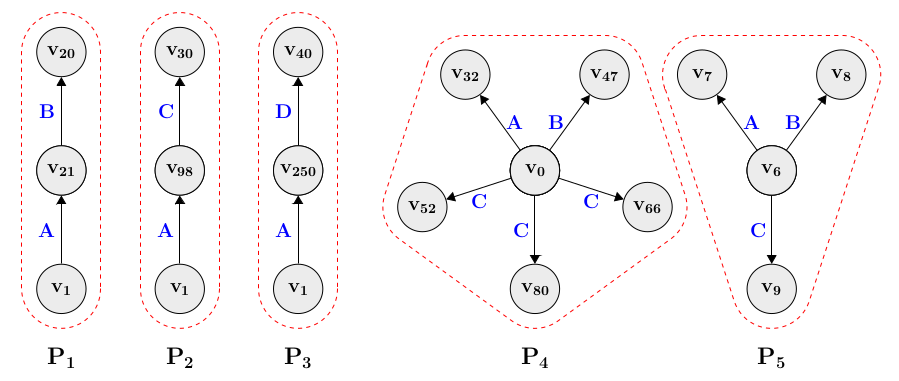
\includegraphics[width=\textwidth]{g_by_q_img}
  \caption{Example of G-by-Q storage representation}
  \label{fig:g_by_q_img}
\end{figure}

This technique proved to be fast and robust against other popular frameworks for querying RDF data, however, the system is complicated - Aluç's implementation was reported to be over 35,000 lines of C++. In this work we aimed to produce simpler contributions. Additionally, the G-by-Q technique is used for point-type queries, which seek to find all instances of certain subgraphs within a graph based on node labels, whereas our contributions are focused on traversal queries, which move through the graph by following edges and making computations based off the node and edge properties.

\section{Graph Processing}

\subsection{Ligra Framework}

Ligra is a lightweight graph processing framework for shared-memory multi-core machines for graph traversal algorithms, such as pagerank and BFS. Ligra takes the form of a simple API of three routines: size, edgeMap and vertexMap, as described in the paper.

\textbf{size}(U) returns the number of vertices in the set U.

\textbf{edgeMap}(G, U, F, C) applies the function F to all edges in G with source vertex in U and target vertex satisfying C.

\textbf{vertexMap}(U, F) applies the function F to every vertex in the set U.

A crucial advantage of the Ligra framework is that in the cases of both edgeMap and vertexMap, the supplied function can run in parallel, however, the user must ensure parallel correctness.

\subsection{Frequency Based Clustering}

Frequency based clustering constitutes physically reorganising the vertex data such that frequently accessed vertices are clustered together. In the case of traversal algorithms, as were studied specifically by this paper, the property by which to cluster vertices is their degree (in- or out-degree depending on the algorithm). By doing this clustering, cache contention between threads is reduced thanks to the improved locality between frequently accessed vertices. This improves cache utilisation and reduces the cycles spent stalled on memory. The authors found that real world graphs often exhibit inherent locality, and disturbing the structure of the vertex data too much causes performance to worsen. They determined that they achieved the best performance when they clustered together vertices at one end of the graph only if their degree exceeded the mean degree across all nodes.

\subsection{CSR segmenting}

This technique, by Kiriansky et al. just like frequency based clustering, aims to optimise the cache performance of a graph algorithm by making random accesses go only to the cache and by making all memory accesses sequential. It does this by working only on a single cache-sized segment of the vertex data at a time. By segmenting the graph into cache-sized subgraphs, all the required vertex data for the processing of a single subgraph can be stored in the cache.

This method requires preprocessing of the adjacency list, followed by the processing of each segment. Segments are processed one at a time, but the computation within the segment is fully parallelised. There is no cache-contention because the threads all share the same read-only working set (vertex data). We can avoid high merging cost after the computations by not using too many segments. The author's did experiments using a high number of segments which fit in the L2 cache, however, the best performance was achieved by using fewer segments, each of which fit in the LLC and contained a large number of edges. After the segments are all processed a low-cost cache-aware merge is used to combine the intermediate results from each segment.

\section{Graph Indices}

\subsection{Space filling curve layouts}

The most famous example of this is the Hilbert Curve, which is a continuous mapping between a number and a point on a 2D square. Numbers which are close by are mapped closely together - in this way the Hilbert ordering of an index of an adjacency list is somewhat locality preserving. We can use a Hilbert ordering in order to improve locality on edge accesses, which therefore leads to improved cache performance.

\chapter{Background}

\label{ch:background}

\section{Database Cracking}

Database cracking was invented by Stratos Idreos as a method of auto-tuning for database kernels by using workload-aware physical restructuring on queried columns. It forms the basis for our contributions in which we apply variants of cracking to graph algorithms with adaptive compression.

\subsection{Cracker Column}

To create an adaptive index for a relational database using a given column, we first copy that column into what is called a cracker column. When executing queries on the chosen column, we execute those queries on the cracker column using modified database operations called cracking operations. In this report we only need to use selection, however cracking can be exploited for insertion, deletion, updates and joins, as well as other operations. We will denote the cracker column by \textit{crk}.

\subsection{Cracker Select}

Initially, there is no information known about the values in the column and their locations. When a ordering query is sent to the cracker column, the column is scanned, and after the scan, all values too small to be selected appear contiguously at the start of the column, followed by all of the selected values, followed by all of the values too large to be selected. Below is an illustration indicating the effect of a cracking operation.

\begin{figure}[h]
  \centering
  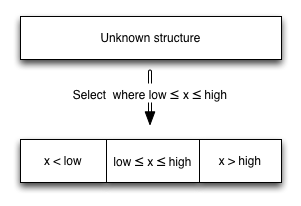
\includegraphics[]{d1_background_cracker_select}
  \caption{Cracking physically restructures the column towards being sorted}
  \label{fig:cracker_select_restructuring}
\end{figure}

Every time we perform a new cracking scan, we learn more information about the values within the column and their associated locations. Our aim is to store and exploit this information to achieve a speed up in performing queries. Notably, selections which occur first in queries are clustered first. In this way the physical layout of the cracker column is adaptive to the workload the database is under. The contiguous regions created through cracking operations are called column fragments.

\subsection{Column Fragments}

Central to the use of cracking is the concept of a column fragment. This represents a contiguous region of the cracker column whose constituent values are potentially bounded by known values. Initially, the entire column represents the only column fragment where there are no bounds yet on the values. However, as queries come in, the scans across the cracker column cause us to gain knowledge about contiguous regions of the column and the values which bound them. As we build up more knowledge about the column, the column fragments get broken up smaller and smaller, meaning that the size of our scans is decreasing as well, given that we are exploiting our knowledge about the fragments and their bounds.

The information about the column fragments is stored in the cracker index.

\subsection{Cracker Index}

The cracker index is a storage data-structure which holds the workload-aware memory about the cracker column fragments. It is denoted \textit{CrkIdx} and is subject to one invariant:

\begin{tcolorbox}
$\texttt{(value, index)}$ $\epsilon$ $\texttt{CrkIdx} \Longrightarrow \forall i < \texttt{index}: crk[i] < \texttt{value}$
\end{tcolorbox}

In plain English, if a \texttt{(value, index)} pair are stored in the cracker index, then all values before \texttt{index} in the cracker column are less than \texttt{value}.

When performing queries, we want to scan only the necessary parts of the column, so we use the information stored in the cracker index to identify the smallest column fragment which is known to contain all of the values we are looking for. After executing such a scan, we put information into the cracker index, effectively breaking up the column fragment we just scanned so that future queries will have to scan less.

\subsection{Tuple Reconstruction}

The cracker column is a copy of the original column, however, the cracking operations only apply to the cracker column, so to reconstruct original tuples based on our results from the cracker column, we use an additional array to act as the mapping between indices in the cracker column and indices in the base (original) columns. This is \textit{late} tuple reconstruction. When the cracker column is initialised, this array is also initialised, its value being an enumeration of the indices from 0 to the length of the column. We call this array the $base\_index$. All restructuring operations that happen to the cracker column also happen to the $base\_index$, in order to maintain the mapping between cracker and base columns.

\subsection{Crack-in-three Algorithm}

The algorithm we describe here as "the cracking algorithm" is actually the "crack in three" variant of the algorithm as described by Idreos. We are using this because for our use case, in which we are always selecting a single node, the crack-in-three algorithm is appropriate, whereas the simpler and faster crack-in-two scan is appropriate when querying for values one side of a given value.

The cracker select operator is called with a low value, $low$ and a high value, $high$, as well as two booleans which indicate the inclusivity of these boundaries. The select returns all the values between $low$ and $high$ in the column using the specified inclusivities.

The cracking algorithm can be grouped into five stages: Setup, tighten, scan, memo and return.

\subsubsection{Stage 1: Setup}

In the first stage of the algorithm, a contiguous section of the column is selected for scanning. If the column hasn't been cracked yet, the cracker column and $base\_index$ are initialised.

Using the arguments, we define the smallest and largest values in the selected range, which depend on the inclusivity of the range at each end.

\begin{tcolorbox}

$\sigma _{min}$ = 
\begin{math}
  \left\{
    \begin{array}{l}
      $low + 1$ \footnote{For integers, the minimum difference between elements is 1, however, for other data types, this may be different. This is discussed further in \ref{ss:perfrag}.} \texttt{, if not inclusive}\\
      $low$ \texttt{, if inclusive}
    \end{array}
  \right.
\end{math}\\
\newline{}\\
$\sigma _{max}$ = 
\begin{math}
  \left\{
    \begin{array}{l}
      $high - 1$ \texttt{, if not inclusive}\\
      $high$ \texttt{, if inclusive}
    \end{array}
  \right.
\end{math}\\
\end{tcolorbox}

We then determine the initial values for the two \textit{edge pointers}. There is a low pointer and a high pointer, which we will denote as $L$ and $H$. These two pointers are subject during the scan to the following invariants.

\begin{tcolorbox}
$(L1)$  $\forall i < L: crk[i] < \sigma _{min}$\\
$(L2)$ $crk[L] \geq \sigma _{min}$\\
$(H1)$ $\forall i > H: crk[i] > \sigma _{max}$\\
$(H2)$ $crk[H] \leq \sigma _{max}$
\end{tcolorbox}

The edge pointers then, bound the region of the cracker column in which all of the sought values lie. It would be optimal to initialise them as \textit{tightly} as possible. When we say \textit{tightly}, what we mean is as far from their associated edge as possible. For $L$ this means as close to the end of the column as possible, and for $H$ this means as close to the head of the column as possible.

To initialise the edge pointers, we search in the cracker index for values which most tightly bound the region of cracker column we have to scan. For $L$, we are looking for the value in the cracker index which is as high as possible, but no more than $low$. If no such value exists, $L$ is intialised at 0. Similarly, for $H$, we seek the value in the cracker index which is as low as possible, but no less than $high$. If no such value exists, $H$ is initialised as $|crk| - 1$.

\subsubsection{Stage 2: Tighten}

The tightening operation involves moving the two edge pointers inwards as far as possible while maintaining their invariants. In practice this is a while loop which checks the associated invariant and if it still holds, tightens the pointer (increment in the case of $L$, decrement in the case of $H$).

During this stage, it is possible to discover that no results exist. For example, if we try to select a value greater than any value in the column, then $L$ will advance all the way off the tail end. For $H$ of course, this happens when we select a value lower than any in the column, with it decrementing off the start of the column. In both of these cases, we return empty results.

Both tightening operations (low-side and high-side) are used in the next stage of the algorithm as well.

\subsubsection{Stage 3: Scan}

At the start of this stage, $L$ is duplicated to produce the \textit{iteration pointer}, denoted $I$, which is subject to a single invariant.

\begin{tcolorbox}
$\forall i: L \leq i < I, \sigma _{min} \leq crk[i] \leq \sigma _{max}$
\end{tcolorbox}

The iteration pointer is used to scan the fragment from $L$ to $H$. As $I$ encounters values within the fragment, it is determined where in the final arrangement they should lie. For example, if the value is less than $\sigma _{min}$, then it is swapped to the value at $L$, and then $L$ is tightened. This maintains the $L$ invariant, while making progress towards the situation in which only selected values are between $L$ and $H$, which is the point at which the scan in finished.

If the value at $I$ is one of the sought values, then $I$ is advanced, which maintains its invariant. Because of this, when $I$ surpasses $H$, this means that all values between $L$ and $H$ inclusive are in the selected range, and by the invariants on $L$ and $H$, every value in the selected range in the column lies between $L$ and $H$, meaning that we're finished with the scan.

Figures \ref{fig:cracking_scan_low_side_1} to \ref{fig:cracking_scan_low_side_3} show the low side swap case from the identification of the swap to the advancement of the low pointer.

\begin{figure}[H]
  \centering
  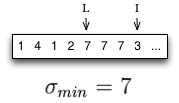
\includegraphics[]{d2_background_cracking_scan_1a}
  \caption{Standard Cracking: Low-side swap recognised}
  \label{fig:cracking_scan_low_side_1}
\end{figure}

\begin{figure}[H]
  \centering
  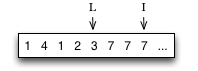
\includegraphics[]{d2_background_cracking_scan_1b}
  \caption{Standard Cracking: Low-side swap performed}
  \label{fig:cracking_scan_low_side_2}
\end{figure}

\begin{figure}[H]
  \centering
  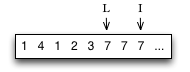
\includegraphics[]{d2_background_cracking_scan_1c}
  \caption{Standard Cracking: Low edge pointer tightened after swap}
  \label{fig:cracking_scan_low_side_3}
\end{figure}

Figures \ref{fig:cracking_scan_high_side_1} to \ref{fig:cracking_scan_high_side_3} show the same thing for the high-side swap.

\begin{figure}[H]
  \centering
  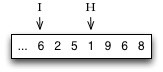
\includegraphics[]{d3_background_cracking_scan_2a}
  \caption{Standard Cracking: High-side swap recognised}
  \label{fig:cracking_scan_high_side_1}
\end{figure}


\begin{figure}[H]
  \centering
  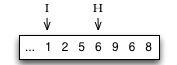
\includegraphics[]{d3_background_cracking_scan_2b}
  \caption{Standard Cracking: High-side swap performed}
  \label{fig:cracking_scan_high_side_2}
\end{figure}

\begin{figure}[H]
  \centering
  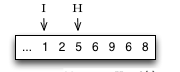
\includegraphics[]{d3_background_cracking_scan_2c}
  \caption{Standard Cracking: High edge pointer tightened after swap}
  \label{fig:cracking_scan_high_side_3}
\end{figure}

\subsubsection{Stage 4: Memo}

At this point, we know for a fact that all values before $L$ in $crk$ are also less than $\sigma _{min}$. This combination of $L$ and $\sigma _{min}$ is enough information to satisfy the main property of the cracker index, so we insert $(L, \sigma _{min})$. Additionally, we know all values before and including $H$ in $crk$ are less than $\sigma _{max}$, so all values before $H+1$ in $crk$ satisfy the required cracker index property. Hence we also insert $(H + 1, \sigma _{max})$.

\subsubsection{Stage 5: Return}

Having acquired the range of cracker column indices in which the selected values lie, we map this back to indices of the original columns using the \texttt{base\_idx} array and retrieve values from the desired column.

\chapter{Adaptive Compression}

\label{ch:adaptivecompression}

\section{Cracking}

In this chapter we examine ways of performing online compression of the adjacency list representing
the graph by modifying the existing cracking algorithms presented by Ideos' et al.. The background
subsection on cracking covers the terms we will use in this chapter to explain the modifications we
made.

Our motivation for applying compression to cracking is to be able to run algorithms faster by exploiting uniform sections of the cracker column.

In this chapter, we will first discuss how we recognize opportunities to compress contiguous, uniform values within the cracker column. Then we will discuss the ways in which the information required to repeatedly exploit these uniform sections of the column can be stored. In the relevant sections and subsections we will describe our implementation of various techniques, which we see the evaluation of the next chapter.

\section{Opportunities}

Given an adjacency list which we are querying using cracking, we can gather information about uniform column-sections with varying eagerness in the course of a cracking scan. We can reserve a decision on compression until we know that an entire column-fragment is compressible, or we can make many small compressions while scanning a fragment of the cracker column.

When we compress only after identifying an entirely uniform column fragment, we call this "per-fragment" compression, because we are compressing entire column-fragments only.

Applying compression during the course of a scan is "eager" compression. Within the space of possibilities for eager compression, we have only explored run-length encoding (RLE) in this project.

\subsection{Per-fragment}

\label{ss:perfrag}

When applying per-fragment compression, we update the cracker index with the boundary values for any created fragment(s) after performing the column scan. If two stored indices are \textit{minimally different}, then we can compress the column in that range, which corresponds to a uniform column-fragment. Minimal difference between stored values is important to per-fragment compression for this reason, and later in this subsection we will explain the concept in more detail.

Advantageously, this method is very easy to implement. One must simply check the boundaries of newly created fragments and determine if any fragments can now be known to be uniform. The cost of this technique on top of normal cracking is a branch in which the cracker index is checked to see if the column fragment under consideration is uniform, meaning the selection can return early.

\subsubsection{Minimal Difference}

We use the phrase \textit{minimally different} to describe two values for which there exists no value between them in the range of values that can be taken for their common type. For example, if we consider the integers, the values 2 and 3 are minimally different, because there exists no integer between these values. For a data-type such as a floating point number, this value will vary depending on the accuracy with which the user wishes to cluster - it may be acceptable to the application that the values 2.33334 and 2.33279 both be considered 2.33, however, unlike in the integer case, there is information being lost during compression, which may not be acceptable to the user. In this case they may opt to use an appropriately fine granularity for the compression according to their application.

\subsection{Run-length Encoding}

Our aim with run length encoded cracking is to be able to speed up the scan by enabling scanning pointers to hop over long runs of the same value. For this, we build and maintain information about all runs of consecutive nodes in the cracker column. This is done inside an array called $run\_lengths$. $run\_lengths[i]$ indicates to a scanning pointer that the next \texttt{i} values (inclusive) are the same, and therefore can be considered together, whether that means that they are hopped over, or swapped away to another part of the column.

Compaction with RLE presents no significant additional difficulties compared to compaction with per-fragment compression. 

The cracker column is scanned both front to back and back to front, therefore it would be preferable
that information be stored such that it can be applied in both scanning directions. For a given run of consecutive values in the cracker column from index $i$ to index $j$ inclusive, the $run\_lengths$ array stores the value $1 + j - i$ at both indices $i$ and $j$, that is, the number of values in the consecutive run.

We also need to maintain the $run\_lengths$ array under the restructuring that takes place during
cracking to make it worthwhile, which requires that we be be careful in maintaining all of the
necessary invariants regarding the position of the two tightening edge pointers used during cracking.

This must also take account of the fact that two runs of different lengths may need to be swapped. When making these swaps of different length runs, the $run\_lengths$ array may have need to have its entries modified in order to retain correctness. In this chapter we discuss two potential approaches to swapping around runs of different lengths within the $run\_lengths$ array.

The first is to swap the entire of the shorter run and modify entries of the $run\_lengths$ array
corresponding to the longer run to maintain consistency after the swap. This means that the longer
run is not fully swapped, so we have called it "underswapping". Underswapping causes the longer run
to get broken up into two runs, one run the same size as the smaller run, which gets swapped entirely with the smaller run, and the other, a run consisting of the entire remainder of the longer run.

The second approach is to swap the entire of the longer run, and pad the shorter run with more elements. This requires the padded elements to have their runs checked and potentially have entries modified, due to the possibility that they are constituents of another run. Due to the fact that the shorter run is swapped with more elements than are actually in that run (by padding), we call this "overswapping". Overswapping maintains runs after they are created, however it is much more complex.

\section{Storage}

After identifying a uniform column section, we have a choice in how to proceed. We can compact the cracker column by deleting duplicated values. Alternatively, we could store the information needed for us to exploit the compression opportunity, without making changing to the physically compacting the data.

\subsection{Compaction}

We describe the choice to delete duplicated values as "compaction". Our implementation uses per-fragment granularity. In our implementation, the cracker column is an array, meaning that to delete arbitrary values requires large copying of memory from the tail side of the array towards the front. Furthermore, when we delete values from the cracker column and copy part of the array towards the head, any entries in the cracker index whose stored pointer will have been offset by the shift must be updated.

It must be possible to reconstruct deleted values after compaction. To solve this, we store information about compacted values, however, we do it indirectly. We store an array called offsets, denoted $ofs$, which holds for each cracker column index, its corresponding index in the base columns. Whenever a value is compressed, that value as well as its minimally different successor value are stored in the cracker index, so when making a selection, if there is only a single instance of the node being selected within the cracker column, we can check to see if it is compressed by comparing its entry in the offsets array with that of the following index. Any compressed value will have a non-consecutive index in its successor, indicating that once there were values between them, which have now been compacted, as illustrated by figure \ref{fig:compaction_causes_non_consecutive_offset_entries}.

\begin{figure}[H]
  \centering
  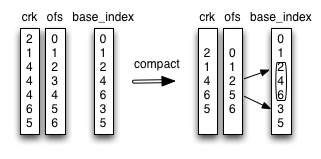
\includegraphics[]{images/d4_compaction_storage}
  \caption{Information about compactions are held in the offset array}
  \label{fig:compaction_causes_non_consecutive_offset_entries}
\end{figure}

The potential advantages of using compaction are that we can fit more edges into memory, that we can improve cache utilization by improving spatial locality among edge clusters within the edge array.

The costs for applying compaction are copying of memory upon compaction, traversing the AVL tree of the cracker index to update all the shifted entries upon compaction, and the maintenance of the  array of offsets.

\subsubsection{Algorithm Overview}

The format of the algorithm is almost the same as standard cracking. After a uniform column fragment is identified, that fragment is compacted. When returning a section of the column, if there are compacted values within the selection, they must be decompressed into the base index by using the offset array.

Figure \ref{fig:compaction_cracker_index_usage} compacting duplicated values results in changes within the cracker index to maintain correctness.

\begin{figure}[H]
  \centering
  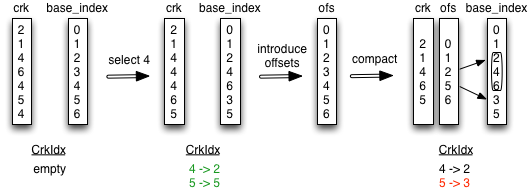
\includegraphics[width=\textwidth]{images/d5_compaction_cracker_index_usage}
  \caption{Compaction causes entries in the cracker index for greater values to be reduced}
  \label{fig:compaction_cracker_index_usage}
\end{figure}

The algorithm starts the same as for standard cracking, however, there is the added introduction of the offset column, which is initialized to 0, because before any compactions have been made, elements in the cracker column are not offset from elements in the base columns. The tightening phase is identical to that of standard cracking.

After the tightening phase, if a single value is identified as the only selected value, then we must check for compression by checking the cracker index to see if this value has been selected (and therefore compressed) before. If so then we can return immediately by decompressing the value at that index in the cracker column.

During the scan, previously compacted values in the cracker column are never swapped around. In our case it is impossible because a previously compressed column fragment will never be contained within a larger range query since our queries are for ranges of just a single node id. Even in the general case, swapping compacted values can be avoided by only cracking the boundary pieces - that is, by not scanning column fragments which are known to be included in the final result anyway, and instead physically reorganizing only the first and last fragments in the selected range.

Single values in the cracker column are swapped around just like for standard cracking, however, the $base\_index$ array may have a different length to the cracker column due to compactions, so the way swaps happen is changed slightly. We use the properties of the offset array to ensure that the correct swaps take place, under the knowledge that no compacted values will ever be swapped.

\begin{tcolorbox}
$\forall i: 0 \leq i < |crk|-1$, $\forall j: ofs[i] \leq j < ofs[i+1]$, $crk[i]$ = $base\_column[base\_index[j]]$
$\forall j: ofs[|crk|-1] \leq j < |base\_column|$, $crk[j]$ = $base\_column[base\_index[|crk|-1]]$
\end{tcolorbox}

With these properties in mind, we swap values in the base index found by passing the relevant pointers through the offset array first. That is, rather than swapping for example the elements at $L$ and $I$, instead we swap the values at $ofs[L]$ and $ofs[I]$.

Immediately after the scan the cracker index is updated and checked for compression opportunities. If the cracker index contains minimally different values, then the values of the smaller run can be compressed, because we know the index in the cracker column before which all entries are exceeded by that value, and also the index after which all values exceed that value. This is the principle of recognition compression, which is discussed in more detail in the next subsection. Figure \ref{fig:compaction_recognition} illustrates this.

\begin{figure}[H]
  \centering
  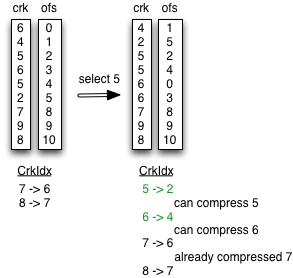
\includegraphics[]{images/d6_compaction_recognition}
  \caption{Minimally different values in the cracker index imply a compression opportunity}
  \label{fig:compaction_recognition}
\end{figure}

If a compression opportunity is found, the compaction is performed. This involves deleting the contiguous indices of the duplicated values for the cracker column and the offsets column. However, when we delete these values, the entries in the cracker column after the compacted value are shifted towards the head of the array. This means that their indices within the cracker column change, and therefore any entries in the cracker index to those values are incorrect. To amend this, all entries in the cracker index whose value is greater than the value being compacted have their index reduced by the number of values compacted. This is because entries in the cracker index with a greater value than the value being compacted necessarily appear later in the column and therefore are shifted during compaction. The reduction is by the number of values compacted, because this is the size of the shift and therefore the size of the required amendment to maintain correctness.

We must take care that the various potential compactions we can perform after the scan do not interfere with one another. Figure \ref{fig:compact_in_correct_order} indicates a scenario in which this can happen. In this diagram, a selection for the value 3 has just finished the scanning phase and is ready to go into compaction. By compacting the lower values first, the implementation must account for headward shifts in the cracker column's values, otherwise the insertion of the next value into the cracker index will be incorrect. In our solution, we address this problem by performing compactions in descending order of the value being compacted.

\begin{figure}[H]
  \centering
  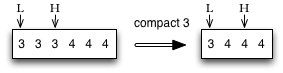
\includegraphics[]{images/d7_compaction_compact_in_correct_order}
  \caption{Compactions can affect each other, headward shifts in later sections of the array must be accounted for.}
  \label{fig:compact_in_correct_order}
\end{figure}

To protect against this problem, we can, as just mentioned, make sure to update pointers appropriately when doing multiple compactions in a single cracker select, or, as we have chosen to do in our implementation, do the compactions always from tail to head, such that there is no potential for interference. Two values are inserted into the cracker index after a selection. The value being selected, and the minimally greater value.

Finally, we return the results to the query. If any compactions took place, we follow the edge pointers from the cracking scan to the offset array and then into the base index, giving us the relevant indices of the base columns.

\subsection{Recognition}

After recognizing a section of column which can be compressed, we need it store this information somewhere in order to later exploit it.

If we are doing per-fragment compression, then we can recognize a compression opportunity when two values are stored in the cracker index which are minimally different. In this case, we need no extra storage - the cracker index contains all the information we need in order to be able to later exploit this.

Otherwise, if we are applying a run-length encoding across the column, we need a separate structure to hold the information about each of the runs, since the compressions are in this case applied at a finer level of granularity than the cracker index is fit to store information about.

The main advantage of recognition versus compaction is that it avoids the various performance costs associated with applying compaction. Additionally, we have found that recognition methods are easier to implement than compaction methods.

To demonstrate an example of how per-fragment recognition compression works, look back to figure \ref{fig:compaction_recognition}. In it, two uniform column fragments are shown at the end of a cracking scan, along with the two edge pointers and the current, unupdated cracker index. It is obvious that the selected column-fragment can be compressed, but the later column-fragment can now also be safely compressed for the same reason. We know in the cracker column the index before which all values are less and the index after which all values are greater, enabling us to exploit this uniform section in the future.

\section{Run-length encoding}

Our aim with run-length encoded (RLE) cracking is to be able to speed up the scan by enabling scanning pointers to hop over long runs of the same value. For this, we build and maintain information about all runs of consecutive nodes in the cracker column. This is done inside an array called $run\_lengths$. $run\_lengths[i]$ indicates to a scanning pointer that the next \texttt{i} values (inclusive) are the same, and therefore can be considered together, whether that means that they are hopped over, or swapped away to another part of the column. Crucially, this applies when encountering $run\_lengths[i]$ in either direction, however, the information about in which direction is not stored, it is assumed that a pointer always visits the "start" of the run in the direction it is traveling. This is an invariant of our implementation.

In compactive RLE, the bi-directionality of the run-lengths stored is trivial, because the duplicated values are all deleted anyway, and only materialize upon tuple reconstruction. However, the complications associated with compaction still apply.

For recognition RLE, the bi-directionality is not a given however, duplicated values are not compacted, meaning that the existence of a run must be marked on both ends, such that a forwards moving edge pointer arrives at the front-side of the run and a backwards moving edge pointer arrives at the tail-side of the run. Figure \ref{fig:rle_bidirectionality} illustrates why duplicating the run-length on both sides of the run is necessary.

\begin{figure}[H]
  \centering
  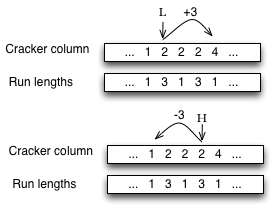
\includegraphics[]{images/d9_rle_bidirectionality}
  \caption{Both forwards and backwards moving pointers need knowledge about runs in order to exploit them}
  \label{fig:rle_bidirectionality}
\end{figure}

Note that the values of $run\_lengths$ within runs is not important, because in a correct implementation we will never read any of those values. In diagrams we will arbitrarily use 1s, although for our implementation any number in the range $[1, rl)$ can occur in $run\_lengths$ within a run of length $rl$.

We also need to maintain the $run\_lengths$ array under the restructuring that takes place during cracking to retain its consistency. We must ensure that the invariants associated with the edge pointers are maintained, and that the properties of $run\_lengths$ are preserved.

This must also take account of the fact that two runs of different length may need to be swapped during the scan. When making these swaps of different length runs, we may need to modify entries of $run\_lengths$ in order to correctly retain its properties. We have studied two approaches to swapping around runs of different lengths during the scanning phase.

The first approach to swapping two runs of different length is to swap the entire of the shorter run and modify entries of $run\_lengths$ corresponding to the longer run to maintain consistency after the swap. This means that the longer run is not fully swapped, so we have called it "underswapping". Underswapping causes the longer run to get broken up into two runs, one run the same size as the smaller run, which gets swapped entirely with the smaller run, and the other, a run consisting of the left-over section of the longer run, which is not swapped. Underswapping aims to be simple to implement while maintaining the scanning benefits of run-length encoding, however runs are often broken and so large gains are not made.

The basic concept is illustrated in figure \ref{fig:rle_underswapping}, in which the outlined green sections are swapped, the outlined red section stays still and the run length values outlined in blue have to be changed to preserve correctness of the $run\_lengths$ array after the swap.

\begin{figure}[H]
  \centering
  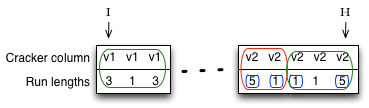
\includegraphics[]{images/d10_rle_underswapping}
  \caption{Example of Underswapping}
  \label{fig:rle_underswapping}
\end{figure}

The second approach is to swap the entire of the longer run, and pad the shorter run with more elements. This requires the padded elements to have their runs checked and potentially have entries modified, due to the possibility that they are constituents of another run. Due to the fact that the shorter run is swapped with more elements than are actually in that run (by padding), we call this "overswapping". Overswapping aims to preserve runs as much as possible, however it is also more complex. The diagram in figure \ref{fig:rle_overswapping} shows an example of using overswapping. The green outlined areas must be swapped, the red areas are also swapped with each other, and run lengths outlined in blue must be changed in order to retain run length correctness after the swap.

\begin{figure}[H]
  \centering
  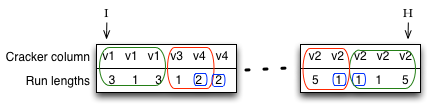
\includegraphics[]{images/d11_rle_overswapping}
  \caption{Example of Overswapping}
  \label{fig:rle_overswapping}
\end{figure}

Later in this section, we will discuss in detail the different cases for swapping around runs of different lengths, for both underswapping and overswapping. First we will look at the sections of algorithm that both of these RLE methods have in common.

\subsubsection{Algorithm Overview}

Both underswapping and overswapping implementations of cracking with RLE recognition compression share most of the algorithm in common. The only differences occur during the scan phase, however we will here describe the rest of the algorithm, which the two implementations share in common.

When the cracker column is initialized as a copy of the original column, $run\_lengths$ is also initialized. Its initial value is an array of the same length as the cracker column filled entirely with 1s.

The edge pointers are initialized from lookups into the cracker index and define the boundaries of the appropriate column-fragment, just like in other variants of the cracking algorithm.

The routines for tightening the pointers are different than for non-RLE variants, because the pointers move by the length of the run they are currently pointing to whenever they are tightened. Additionally, while tightening the edge pointers, we are looking for opportunities to build up and mark runs of duplicated values that they encounter.

When tightening the edge pointers in the tightening phase, we move pointers by jumping over each run, as well as building them up as we encounter them, while making sure to avoid under/overflow for cases where the value being sought isn't present. The way a run is built up during the tightening phase, using the low side pointer as an example, is shown in figure \ref{fig:rle_run_building}.

\begin{figure}[H]
  \centering
  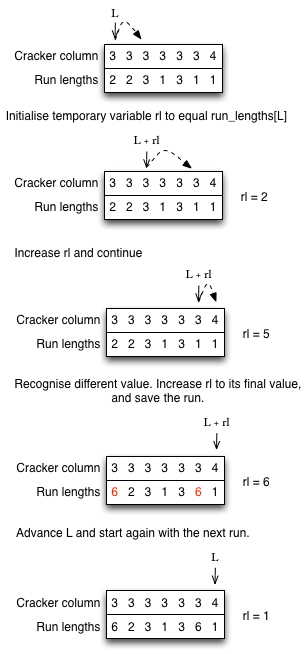
\includegraphics[]{images/d12_rle_run_building}
  \caption{Run building with the low edge pointer}
  \label{fig:rle_run_building}
\end{figure}

The case of swapping runs of different lengths between the low and iteration pointers is the same for both underswapping and overswapping, because we have the knowledge that the values at the indices in the range $[I, L)$ are all the value being queried for. This means that we can immediately make a run out of it and do as big a swap as possible, advancing the pointers as much as possible. We did experiment with using the strict underswapping and overswapping methods for these stages, however we found that the exploiting the information we knew about the intermediate values between $I$ and $L$ gave better performance than either of them. Later in this subsection we describe the low-side swaps in more detail.

When the iteration pointer is to be advanced during the scan, we can choose to try to build runs during the advancement, or not. After trialling both methods on our generated datasets, we found that trying to build runs causes the algorithm to slow down, so our final implementations don't do that.

Also during the scan, the tightening of pointers after making swaps is the same as for standard cracking, including the fact that if the low edge pointer overtakes the iteration pointer during tightening, the iteration pointer catches up immediately.

After the scan, we check that values were indeed selected - if the low edge pointer has surpassed the high edge pointer, then we know from their relative invariants that the sought value isn't present in the column. Figure \ref{fig:edge_pointers_pass_each_other} illustrates this fact.

\begin{figure}[H]
  \centering
  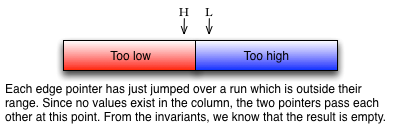
\includegraphics[]{images/d13_edge_pointers_pass_each_other}
  \caption{Two tessellating runs, neither of which are selected, form the boundary at which the edge pointers pass each other in a query returning no results.}
  \label{fig:edge_pointers_pass_each_other}
\end{figure}

Once the scan is finished, we combine into a single run the entire resultant fragment containing all instances of the value to be returned. We know this is the case for the same reason as when we do per-fragment compression. The insertion into the cracker index and returning of values is the same as for standard cracking.

\subsubsection{Low side swaps}

If the two runs to be swapped are the same length, then we can swap them immediately and entirely without doing anything else, because no runs are going to be invalidated and so none need to be edited.

If however they are different lengths, then we first change the situation in order to eliminate the possibility of having to deal with the situation in which values used to pad the shorter run spill into the longer run, creating an overlap. The change we make uses our knowledge that all the values of the cracker column lying within the index range $[L, I)$ are the selected value. We combine all of these values into a single run, resulting in the two runs to be swapped having a border just before the iteration pointer.

Our aim is to make the swap while preserving as much of the longer run as possible. To do this, we swap the entirety of the smaller run and edit the $run\_lengths$ array so that consistency is maintained.

\subsubsection{Low side swaps: Iteration run shorter}

Figure \ref{fig:rle_lowside_1a} shows the situation. The swap we intend to make is outlined in green and the run lengths to be amended are outlined in blue. We must ensure that after this swap takes place the properties of $run\_lengths$ are preserved.

\begin{figure}[H]
  \centering
  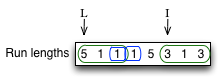
\includegraphics[]{images/d14_rle_lowside_1a}
  \caption{RLE low side swap, iteration run shorter: Swap recognized}
  \label{fig:rle_lowside_1a}
\end{figure}

Since we are swapping the full iteration pointer side run, we know that the last element getting swapped of those will be ending up at the tail end of our final run of selected values. Therefore we amend this entry in $run\_lengths$ with the number of values, which is equal to the difference between the two pointers, since all the values between them will constitute this run. Similarly, we know the element which will be at the start of the final run immediately follows the last element being swapped with the iteration run, so we amend that entry in $run\_lengths$ with the difference between the pointers as well. These amendments to $run\_lengths$ are shown in figure \ref{fig:rle_lowside_1b}.

\begin{figure}[H]
  \centering
  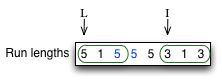
\includegraphics[]{images/d14_rle_lowside_1b}
  \caption{RLE low side swap, iteration run shorter: Run lengths entries amended}
  \label{fig:rle_lowside_1b}
\end{figure}

Having amended $run\_lengths$ appropriately, we can perform the full swap of the iteration side run with the appropriate number of elements from the low edge pointer, knowing that the resulting entries in the cracker column and $run\_lengths$ array will be consistent. Figure \ref{fig:rle_lowside_1c} shows the run lengths array after the swaps are completed.

\begin{figure}[H]
  \centering
  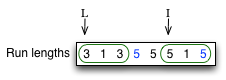
\includegraphics[]{images/d14_rle_lowside_1c}
  \caption{RLE low side swap, iteration run shorter: Swaps completed}
  \label{fig:rle_lowside_1c}
\end{figure}

At this point, we must advance the pointers to make progress in the scan. We know that the run we just swapped down to the low edge pointer contains values less than the selected node id, so the low edge pointer should be advanced beyond them. Also, the iteration pointer is now in the middle of a run, which is dangerous, so we get it out of there by advancing it to the end of that run. We don't swap it to the beginning because we know that it is a run containing the node id under selection - no need to scan it. The diagram in figure \ref{fig:rle_lowside_1d} demonstrates the advancing of the pointers.

\begin{figure}[H]
  \centering
  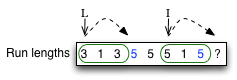
\includegraphics[]{images/d14_rle_lowside_1d}
  \caption{RLE low side swap, iteration run shorter: Pointers tightened}
  \label{fig:rle_lowside_1d}
\end{figure}

\subsubsection{Low side swaps: Iteration run longer}

In this situation, the shorter low-side run must be swapped to the end of the iteration run. We must again edit $run\_lengths$ to maintain consistency, as we can be seen from figure \ref{fig:rle_lowside_2a}.

\begin{figure}[H]
  \centering
  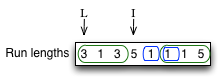
\includegraphics[]{images/d15_rle_lowside_2a}
  \caption{RLE low side swap, iteration run shorter: Swap recognized}
  \label{fig:rle_lowside_2a}
\end{figure}

The first element of the iteration run swapped with the low-side run must have its run-length changed, as well as the last element of the iteration run that is not swapped, so that after the swap, both sides of the run are still marked. The arithmetic for finding these positions is straightforward. Figure \ref{fig:rle_lowside_2b} shows the same situation as above but with the necessary amendments.

\begin{figure}[H]
  \centering
  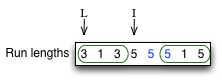
\includegraphics[]{images/d15_rle_lowside_2b}
  \caption{RLE low side swap, iteration run longer: Run lengths entries amended}
  \label{fig:rle_lowside_2b}
\end{figure}

After the amendments, the entire low-side run is swapped to the end of the iteration run, and the updated run markings mean that the iteration run is again wholly preserved, which you can see in the figure \ref{fig:rle_lowside_2c} .

\begin{figure}[H]
  \centering
  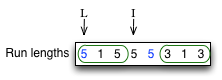
\includegraphics[]{images/d15_rle_lowside_2c}
  \caption{RLE low side swap, iteration run longer: Swaps completed}
  \label{fig:rle_lowside_2c}
\end{figure}

Finally, the pointers must be updated. The low pointer can hop over the swapped back run, since we know that its duplicated value is less than the selected value. The iteration pointer moves to the start of the run that was swapped forwards, the position of which was calculated earlier. Figure \ref{fig:rle_lowside_2d} shows how the pointers are updated.

\begin{figure}[H]
  \centering
  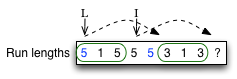
\includegraphics[]{images/d15_rle_lowside_2d}
  \caption{RLE low side swap, iteration run longer: Pointers advanced}
  \label{fig:rle_lowside_2d}
\end{figure}

\subsection{Underswapping Scan}

Underswapping is the simpler of the two approaches, because it has fewer edge cases to consider. We have only to amend the two pieces of the broken longer run before swapping all the values from the smaller run across to the equally sized run just created from a piece of the longer run. This method wastes some information we have acquired, but is fairly simple.

Within the cracking scan, if the run at the iteration pointer is to be swapped, it will either be swapped with the run at the low edge pointer or the high edge pointer. If the runs have equal length, they can be swapped immediately with no further amendments. Otherwise, the run which is longer can either be the run getting swapped towards the middle or towards the edge.

Under the following headers, we describe and illustrate the algorithm's behavior given the circumstance of the run at the iteration pointer. The two cases are all fairly similar and straightforward. We have lay them out in series of diagrams, starting at the initial situation, and ending with the runs swapped and the pointers appropriately tightened for the next iteration.

\subsubsection{High side swaps: Iteration run shorter}

The diagram in figure \ref{fig:underswapping_1a} shows the situation once we have identified that we are doing a high-side swap and the iteration run is shorter. The sections to be swapped are outlined in green and the run lengths which need to be amended are outlined in blue. We do not know about the intermediate values between the two runs, if there are any, so we have included an ellipsis in the depiction of the column to indicate these values.

\begin{figure}[H]
  \centering
  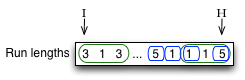
\includegraphics[]{images/d18_underswapping_1a}
  \caption{Underswapping high side run, iteration run shorter: Swap recognized}
  \label{fig:underswapping_1a}
\end{figure}

Figure \ref{fig:underswapping_1b} shows the amendments, which are shown with blue font. Due to underswapping, we can see that the long run of 5 has been broken into a run of 2 and a run of 3 in order to facilitate the swap. Below the run lengths array in the diagram is the cracker column, which we have filled with two generic values - $i$ for the duplicated value in the iteration run, and $h$, the duplicated value in the high-side run.

\begin{figure}[H]
  \centering
  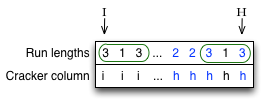
\includegraphics[]{images/d18_underswapping_1b}
  \caption{Underswapping high side run, iteration run shorter: Run lengths entries amended}
  \label{fig:underswapping_1b}
\end{figure}

After the swap, the values are moved and the correctness of run lengths and the cracker column is maintained from the amendments. We can also see that the run of $i$, known to be too great to be included in the selection, has been moved to the high-pointer and is ready to be hopped over.

\begin{figure}[H]
  \centering
  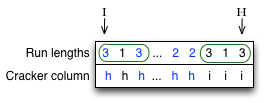
\includegraphics[]{images/d18_underswapping_1c}
  \caption{Underswapping high side run, iteration run shorter: Swaps completed}
  \label{fig:underswapping_1c}
\end{figure}

Finally, in figure \ref{fig:underswapping_1d} we show the tightening of the high pointer in which it hops over the swapped-up run.

\begin{figure}[H]
  \centering
  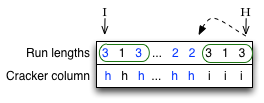
\includegraphics[]{images/d18_underswapping_1d}
  \caption{Underswapping high side run, iteration run shorter: High pointer tightened}
  \label{fig:underswapping_1d}
\end{figure}

\subsubsection{High side swaps: Iteration run longer}

As before, the sections to be swapped are outlined in green and the run lengths which need to be amended are outlined in blue. The ellipsis is also used in the same way as it was under the previous header. The situation is shown in figure \ref{fig:underswapping_2a}.

\begin{figure}[H]
  \centering
  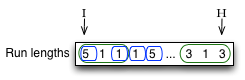
\includegraphics[]{images/d19_underswapping_2a}
  \caption{Underswapping high side run, iteration run longer: Swap recognized}
  \label{fig:underswapping_2a}
\end{figure}

Figure \ref{fig:underswapping_2b} shows the arrays after amending the necessary run lengths.

\begin{figure}[H]
  \centering
  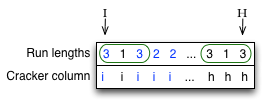
\includegraphics[]{images/d19_underswapping_2b}
  \caption{Underswapping high side run, iteration run longer: Run lengths amended}
  \label{fig:underswapping_2b}
\end{figure}

The amendments mean that after the swaps the runs are still all correct, as shown in figure \ref{fig:underswapping_2c}.

\begin{figure}[H]
  \centering
  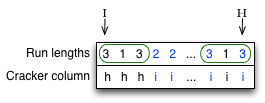
\includegraphics[]{images/d19_underswapping_2c}
  \caption{Underswapping high side run, iteration run longer: Swaps completed}
  \label{fig:underswapping_2c}
\end{figure}

Finally, the high edge pointer hops over the swapped up run to tighten the region to scan. This is shown in the diagram in figure \ref{fig:underswapping_2d}.

\begin{figure}[H]
  \centering
  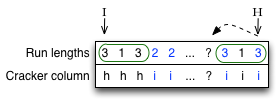
\includegraphics[]{images/d19_underswapping_2d}
  \caption{Underswapping high side run, iteration run longer: High pointer tightened}
  \label{fig:underswapping_2d}
\end{figure}

\subsection{Overswapping Scan}

When overswapping, we swap the entire of the longer run, and pad the shorter run to length. The runs within the padding must be amended to remain consistent, and if the padding contains partial runs, then those runs must be amended outside the padding as well to remain consistent after the swap. Additionally, if the padding causes the two swapped regions to overlap, then we don't have to swap all of the values - a saving that requires us to also make updates into $run\_lengths$ to preserve correctness.

Unlike in the low-side swap case, we know nothing about the values between the iteration pointer and high pointer, other than that the value at the high pointer is not greater than \textit{x}.

\subsubsection{High side swaps}

As with low side swaps, when the runs are the same length, we can immediately swap them without any fuss and advance the edge pointer appropriately.

For high side swaps of unequal length, we have no information about the intermediate values between the two runs being swapped, therefore we have to manage the padding and ensure that no inconsistencies are introduced into $run\_lengths$ as a result. This includes the possibility that the padding may spill into the longer run and the possibility that the padding may form part of another separate run, causing that run to potentially become broken apart. We describe the first of these possibilities as "overlapping" because the padded shorter run overlaps with the longer run. The second we describe as the padding having a remainder, requiring amendments to $run\_lengths$.

In our description of high-side overswapping, we will first describe the case in which the padding overlaps with the longer run. Then to describe non-overlapping padding, we will describe the strategy we used to deal with padding which has a remainder, followed by an explanation of the swaps which take place after the padding has been prepared.

\subsubsection{Overlapping}

Figure \ref{fig:overswapping_overlapping} is an illustration of the two possible cases of overlapping when swapping high-side runs. The values in the longer run which are also part of the padding are shown in red font.

\begin{figure}[H]
  \centering
  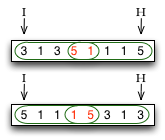
\includegraphics[]{images/d20_overswapping_overlapping}
  \caption{Padding can overlap with the longer run.}
  \label{fig:overswapping_overlapping}
\end{figure}

This problem is just like the low-side swap cases, but with slightly different arithmetic because $H$ points to the tail end of its run. Because we assume that the $run\_lengths$ array is consistent, we know that we can take padding right up to the border with the other run and know that there is no possibility that the padding has any remainder. From this position we swap all the values between the iteration and high pointers except for the overlapping region, after making some adjustments in the longer run.

After the amendments are made we swap the two sections, the longer run aligns so consistency is preserved and the longer run is fully preserved.

\subsubsection{Padding Remainder}

The problem here is that the padding may contain for example two out of three elements of a run, meaning that if the padding gets swapped, the run will be broken. The padding may contain multiple runs - we need only check the last one. The ideal case is for the last run in the padding to be entirely contained within it, that is, the padding has no remainder.

Our approach to fixing padding remainder is to use underswapping. We break the padded run into a run inside the padding and a run outside the padding.

The implementation of this method is that we first initialize a padding pointer, with a view to move it through the padding until finding the last run. We then check if the padding has a remainder or not. If it doesn't, we don't need to do anything, otherwise, we fix the remainder into two runs as described in the previous paragraph.

Although the padding extends in different directions depending on which side it's on, the only thing that changes is the necessary arithmetic to fix the remainder if there is one, and to calculate the location of the swaps. We illustrate in figure \ref{fig:padding_remainder} the amendments that must be made due to the padding remainder both in the case where the iteration run is longer and in the case where the high run is longer. 

\begin{figure}[H]
  \centering
  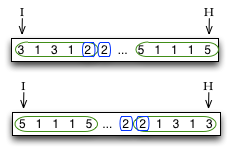
\includegraphics[]{images/d22_padding_remainder}
  \caption{Padding can contain partial runs which must be amended.}
  \label{fig:padding_remainder}
\end{figure}

\subsubsection{Padding Swaps}

At the stage at which we start to consider doing swaps, we have two equal length sections of column. The longer run is one of these sections, it is uniform. The other contains a run whose value we know and want to swap to the far side of the longer run, plus some padding to bring it up to length. The padding contains only whole runs and no runs will be broken by swapping it away, either by coincidence or because we have explicitly amended it.

We consider both of the two sections in two different parts. The shorter run, and the part of the longer run which will be swapped with it, are both one part, which we call the main part, because it constitutes the reason why we are doing the swap in the first place. The padding of the shorter run, and the corresponding part of the longer run we call the padding part, or just "the padding". In both the case where the iteration run is longer and where it is shorter, the padding is towards the middle-ground between the iteration and high pointers, as you can see from figure \ref{fig:padding_remainder}. After the swap therefore, the relative order of the main and padding parts will be swapped, meaning that we will have to make amendments in the longer run in order to preserve it. The run length entries which must be amended are outlined in blue in figure \ref{fig:padding_swaps_amendments}.

\begin{figure}[H]
  \centering
  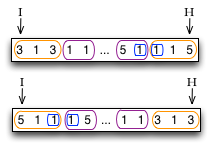
\includegraphics[]{images/d23_padding_swaps_amendments}
  \caption{Amendments in the runs for swapping both the main and padding parts during a high-side overswap.}
  \label{fig:padding_swaps_amendments}
\end{figure}

After the swap we are left with the iteration run swapped up and the $run\_lengths$ array in a correct state. Finally we tighten the high pointer by hopping it over the run that got swapped up. This is illustrated in figure \ref{fig:padding_swaps_done}.

\begin{figure}[H]
  \centering
  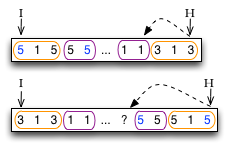
\includegraphics[]{images/d25_padding_swaps_done}
  \caption{Tightening the high pointer after a completed high-side overswap.}
  \label{fig:padding_swaps_done}
\end{figure}
\chapter{Evaluation}

\label{ch:evaluation}

\section{Experimental Setup}

The experiments were performed on the department of computing lab machines, $sprite30$ and $sprite29$. These machines have a "HP EliteDesk 800 G2 TWR, Intel Core i7-6700 3.40GHz" CPU and have 16GB of RAM.

\section{Datasets}

\subsection{LDBC Social Network Benchmark Data Generator}

To test our work, we have used the LDBC-SNB DataGen program \cite{Erling:2015:LSN:2723372.2742786}, which generates a social network graph to a number of scale factors. We used scale factors 1, 3 and 10. We would have used larger data but for the size of the machine we performed our experiments with. The number of nodes and edges in these graphs is shown in table \ref{tab:datasets_table}.

\begin{table}[H]
    \centering
    \begin{tabular}{| l | l | l |}
    \hline
    Scale Factor & Nodes & Edges \\ \hline
    1 & 9893 & 180624 \\ \hline
    3 & 24329 & 565248 \\ \hline
    10 & 65646 & 1938517 \\
    \hline
    \end{tabular}
    \caption{LDBC-SNB generated datasets}
    \label{tab:datasets_table}
\end{table}

A major use-case for adaptive indexing on graph data is the prospect of finding trends within a social network. When something happens in the news, for example, the workload changes, requiring a new index to improve performance. We have used a simple popularity/trend-analysis measure in pagerank ("personrank" in our case) to assess the performance of our system.

In this network, people are nodes and their relationships are edges. The node ids are unchanged from the data generation, they are not mapped onto consecutive integers from 0.

\subsection{Randomly Generated Trees}

We wished to find the break-even point of up-front sorting versus our implementations, so to support this, we used breadth-first search on randomly generated trees. To find the "break-even point", we find the time it takes to sort the edge array using quicksort \cite{doi:10.1093/comjnl/5.1.10} and then count the number of queries the cracking implementation has already answered in that time. This is used to determine the gains we can make by using adaptive indexing versus using offline index creation, that is, up-front sorting.

\section{Graph Algorithms}

\subsection{Breadth First Search}

Breadth first search, or BFS, involves choosing a starting node as the sole member of a frontier, which then expands in iterations in which members of the frontier append their out-neighbours which have not yet been visited to the frontier, and remove themselves. This continues until all vertices have been visited.

The most important factor for us in considering BFS is that it queries the outgoing edges of each node just once, meaning that compressed column fragments are never revisited during the course of the algorithm. For this reason we believe it provides an appropriate lower bound on the break-even point.

\subsection{Pagerank}

Pagerank \cite{ilprints422} is a famous algorithm which stores a rank for each vertex and iteratively updates the values across the entire graph. All nodes are initialized with a rank of $\frac{1}{|V|}$. During each iteration, each node inherits from all of its in-neighbours a contribution of their pagerank divided by their out-degree. This value is then multiplied by a damping factor and then added to a base value to give the updated rank. The base value is defined as $\frac{1 - d}{|V|}$.

In pagerank, every iteration considers all of the vertices and edges in the graph, and so over an execution of many iterations, any clustering or compression will see further benefits compared to BFS.

To benchmark our contributions, we have implemented pagerank as an equivalent "personrank" for the generated social network.

\section{Systems under Comparison}

The purpose of this project is not to create the fastest system, but to assess the applicability towards graph processing of compression-based variants of cracking. To ensure that our experiments fairly reflect this, we have chosen to compare our single-threaded cracking implementation to other single-threaded solutions. Predicated and vectorized implementations of cracking have been done and been shown to be highly effective for improving the CPU efficiency of cracking against the original algorithm \cite{Pirk:2014:DCF:2619228.2619232}, however, we have not applied these improvements to our algorithm. This is not a problem because our work is concerned primarily with the fundamental differences between standard cracking and cracking with adaptive compression, rather than optimizing them especially, although we touch on potential optimizations in our discussion of future work.

With that in mind, we have tested our system against the standard cracking algorithm and against upfront quicksort. The reason we have chosen quicksort specifically is for its similarity to cracking, in that it uses pivots to partially sort column sections. Compare this to cracking, which uses pivots to partition the column towards being fully sorted.

Our contributions featured variations in two dimensions: Opportunities to compress and storage of compression information. We have implemented per-fragment compaction, per-fragment recognition, underswapping RLE recognition and overswapping RLE recognition. The reason we decided not to implement compaction with RLE compression is that it seemed clear from the disappointing results of per-fragment compaction that it would not be worth it.

\section{Results}

\subsection{Personrank}

Using data generated by the LDBC-SNB at scale factors of 1, 3 and 10, we measured the wall-clock time to completion of pagerank implementations using each adaptive indexing technique. We have also included the results for an implementation using upfront quicksort.

For each of the three graphs, we ran pagerank over 50 and 100 iterations for every method. Each result is averaged over 10 runs. Blue and red represent the results over 50 and 100 iterations respectively.

\begin{figure}[H]
  \centering
  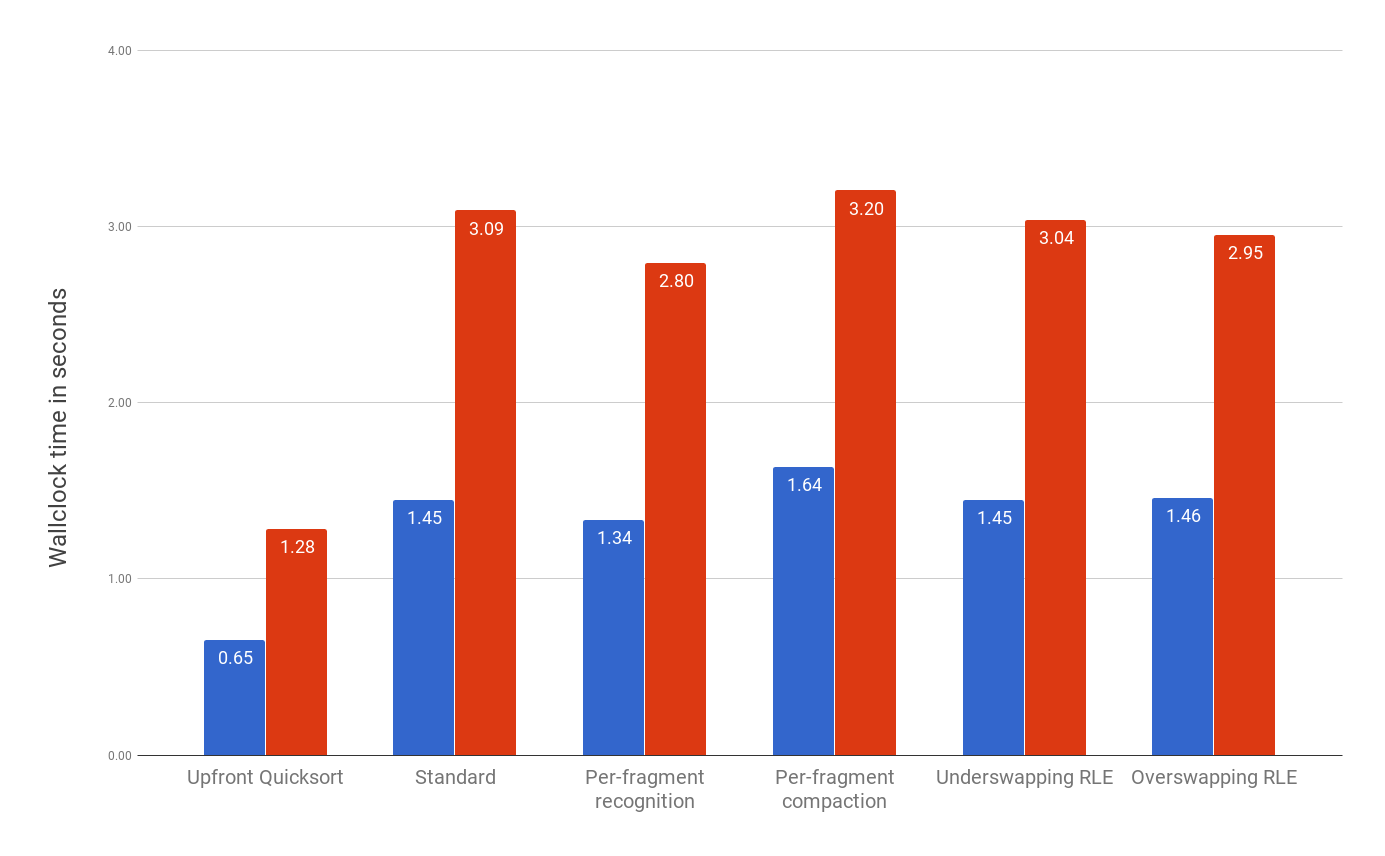
\includegraphics[width=\textwidth]{images/personrankSF1}
  \caption{Personrank execution times for the SF1 social network graph}
  \label{fig:personranksf1}
\end{figure}

\begin{figure}[H]
  \centering
  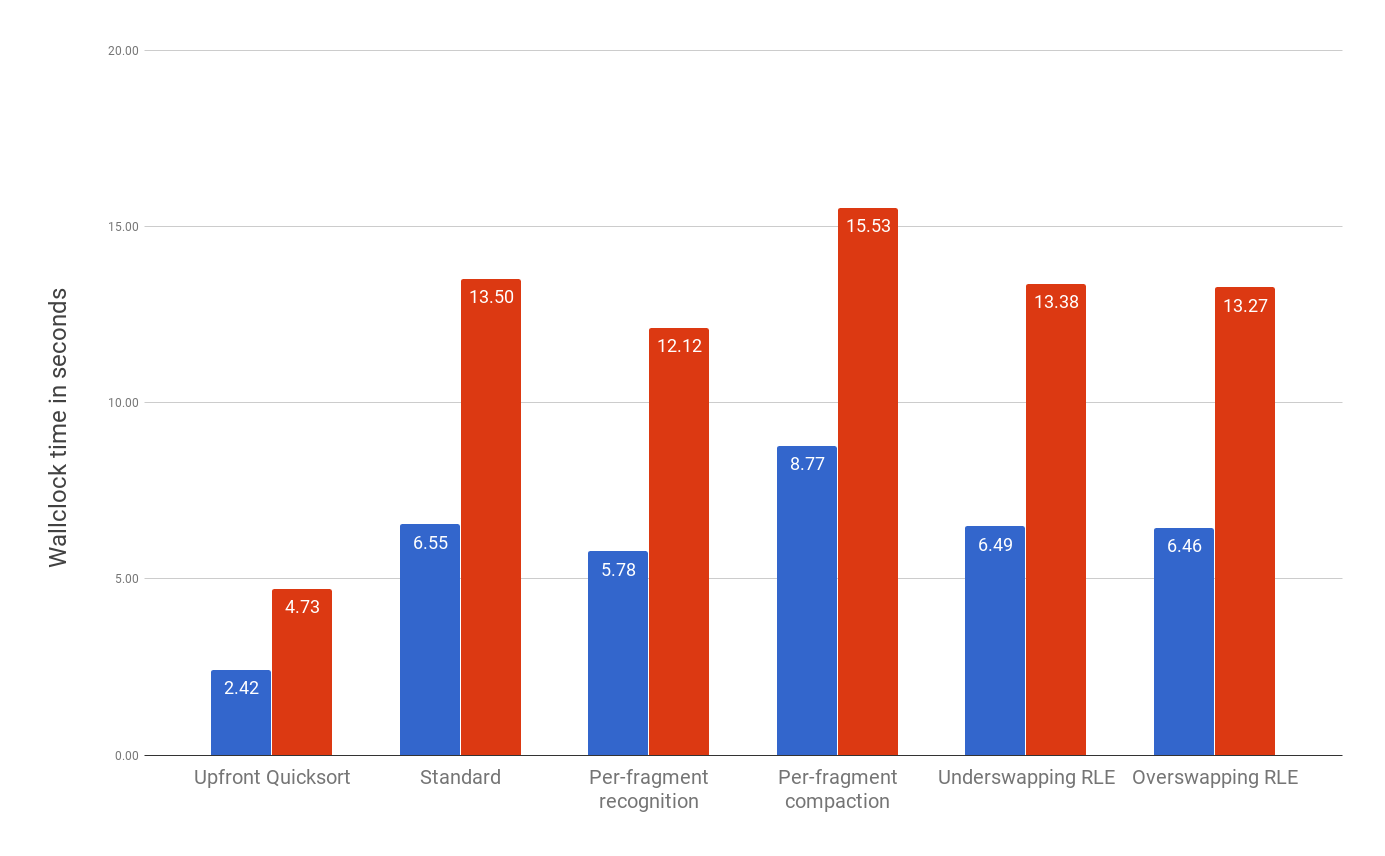
\includegraphics[width=\textwidth]{images/personrankSF3}
  \caption{Personrank execution times for the SF3 social network graph}
  \label{fig:personranksf3}
\end{figure}

\begin{figure}[H]
  \centering
  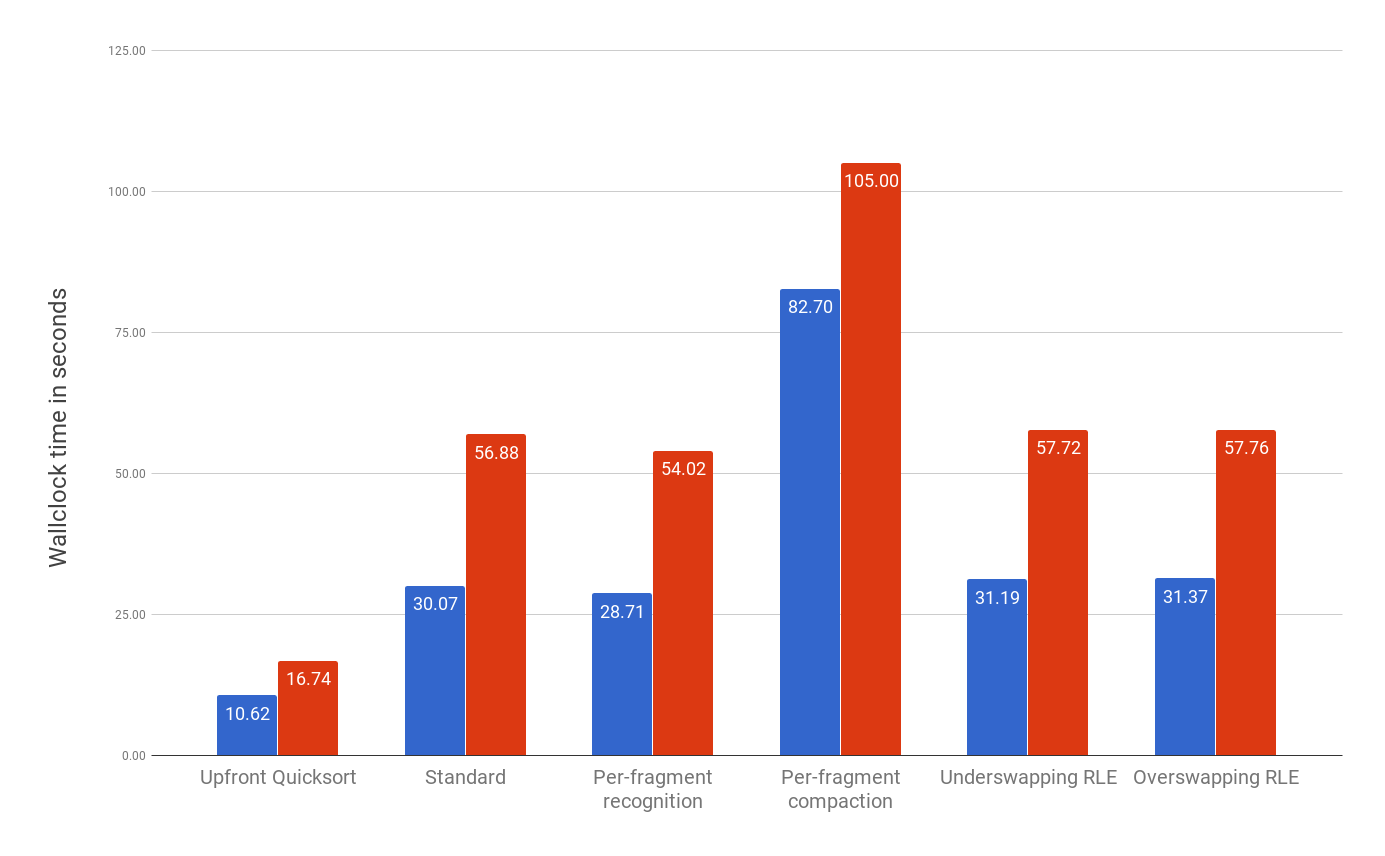
\includegraphics[width=\textwidth]{images/personrankSF10}
  \caption{Personrank execution times for the SF10 social network graph}
  \label{fig:personranksf10}
\end{figure}

Our experiments showed that our implementation of compaction is always the slowest, regardless of data size or the number of iterations. This is due to the prohibitively high costs associated with the constant copying of memory which this technique depends on.

We also showed however, that per-fragment recognition was always the fastest. This is because, by recognizing a uniform column-fragment, we can avoid doing any scanning at all. This optimization to the original algorithm yielded a small average speedup across our six reported executions of 8.1$\%$.

The two RLE methods we developed showed promise. Across our reported executions, they were faster than standard cracking as often as they were slower. We found very little difference in performance between underswapping and overswapping, although this is likely to be because they are inherently very similar, differing only in the way they perform high-side swaps of two runs of different lengths - a case which is evidently not encountered enough to show any sizable performance difference between the two different implementations of that case.

\subsection{Break-even Point}

Using randomly generated trees, we ran BFS using each adaptive method and counted how many cracking queries were completed in the same amount of time as it took to sort the tree using quicksort.

The reason we chose to do BFS on trees, is that it represents a case in which every query is guaranteed to be doing a scan and not returning compressed values. We did this in order to assess how much of an impact on the break-even performance and early-scanning speed our changes had to the original cracking algorithm.

We evaluated the break-even point for trees of size 100,000, 500,000 and 1,000,000 (number of nodes), averaged over 10 runs, with a new tree for each run. Our results are shown in figure \ref{fig:breakeven}. Blue, red and yellow represent the results for the trees with 100,000, 500,000 and 1,000,000 nodes respectively.

\begin{figure}[h]
  \centering
  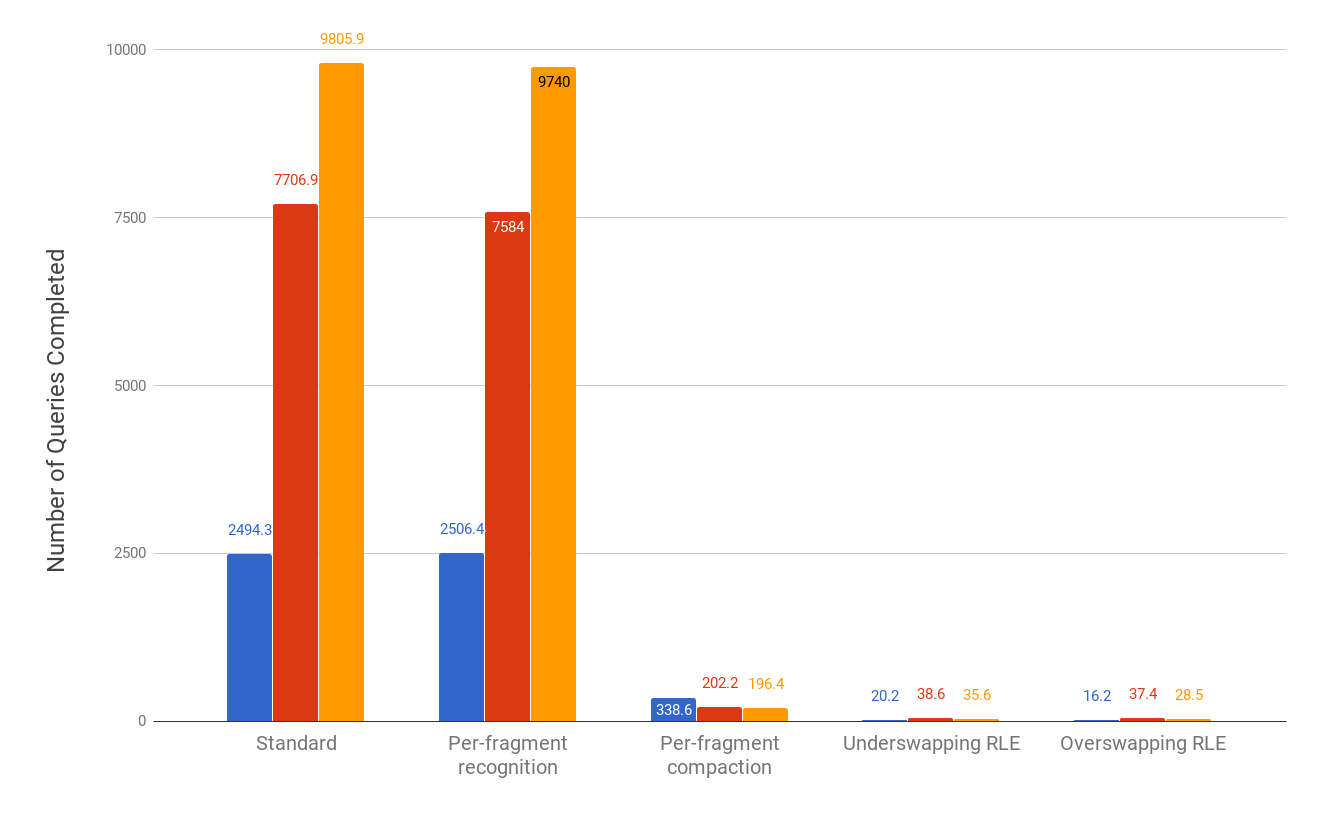
\includegraphics[width=\textwidth]{images/breakeven}
  \caption{Break-even point for each studied adaptive technique}
  \label{fig:breakeven}
\end{figure}

Compaction performed poorly compared to standard cracking in this test. We see that with greater data size, the number of queries ran by compaction in the same time as it took to sort the array decreases. This makes sense given that the primary cost factor in compaction is the copying of memory. As the size of the array increases and the number of copied values increases, so the performance during early queries will decrease.

Per-fragment recognition makes no changes to the cracking scan, and so it makes sense that there would be little difference in the break-even point compared to standard cracking, regardless of the data size.

The two RLE cracking variants actually change the implementation of the scan - they perform extra work to build and maintain knowledge about runs in exchange for the ability to exploit this knowledge. In the early queries we expect the costs to outweigh the benefits, because at the start, there is no run-length information to exploit, but at the same time there is a lot of new information to build and write into memory, which is expensive. This results in a significantly higher relative cost for early queries when using RLE cracking, causing the break-even point to be dramatically lower. This is unfortunate, because one of the main advantages of using cracking over a non-adaptive indexing technique is that it is lightweight - a property lost by performing expensive run-length encoding in early queries.

Compared to overswapping, underswapping performs less work during high-side swapping. It has fewer branches because it does not have to deal with padding or overlapping. The earliest queries perform the largest scans and therefore perform the most swaps. It therefore makes sense that the relative advantage underswapping has in performing less work during swapping would be most evident in the earliest queries.

\subsection{Summary}

\begin{itemize}
\item \textbf{Per-fragment Compaction}: This method was quite disappointing, although it cannot be said that it was unexpected. The costs of deleting arbitrary elements from an array and copying the non-contiguous data towards the head are too high to make this a viable technique.
\item \textbf{Per-fragment Recognition}: By recognizing uniform column pieces using the invariants of the cracker index, we can prevent unnecessary scans, which improves performance. We showed that per-fragment recognition is an effective way to improve the performance of cracking as an adaptive index on an edge-array representing a graph.
\item \textbf{RLE}: We showed that run-length encoding an edge array during cracking is a technique that performs similarly to standard cracking in terms of overall speed, but is a far less lightweight operation.
\end{itemize}
\chapter{Conclusion}

\label{ch:conclusions}

\section{Summary of Contributions}

\section{Applications}

\section{Future Work}

\input{appendix/appendix.tex}

\renewcommand\bibname{References}
\bibliographystyle{abbrv}
\bibliography{bibs/refs}

\end{document}